\documentclass{standalone}
\usepackage{tikz}
\usepackage{amsmath,amssymb,bm}
\usetikzlibrary{arrows.meta,positioning,fit}

\begin{document}
	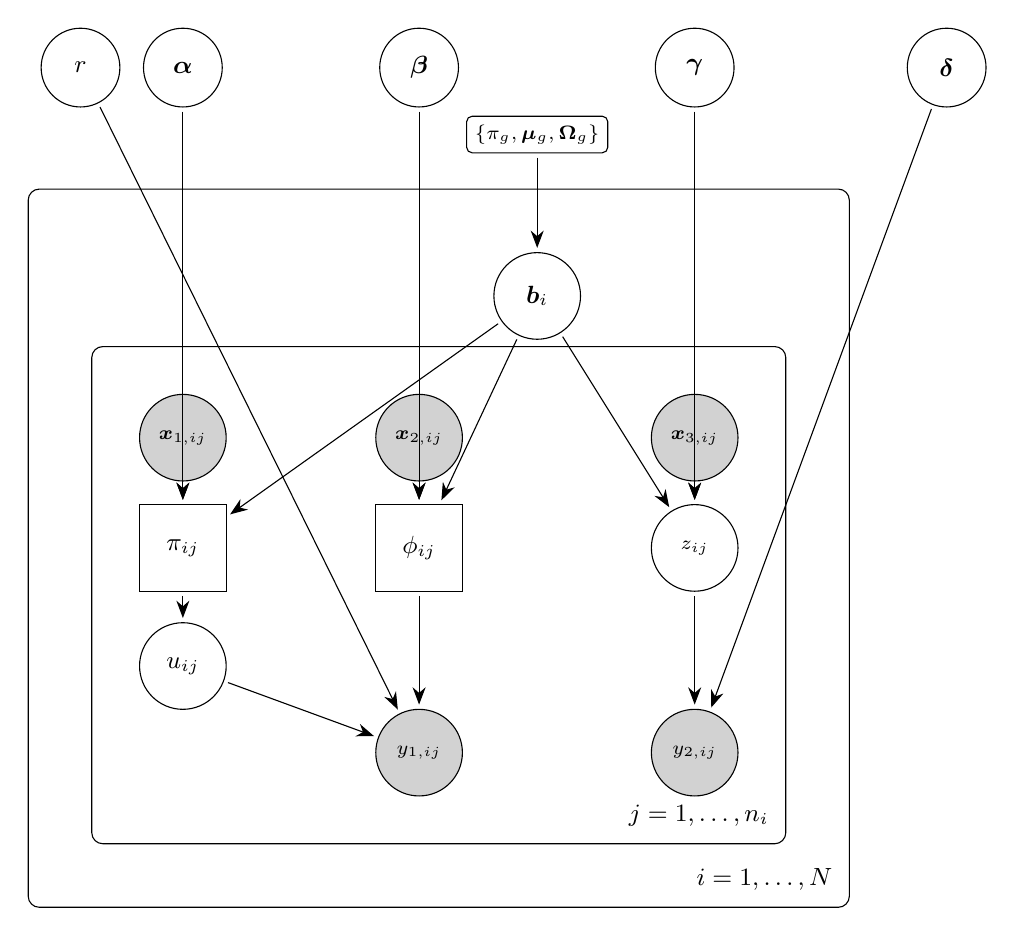
\begin{tikzpicture}[
		>={Stealth[length=2.2mm]},
		latent/.style={circle,draw,minimum size=11mm,inner sep=1pt,font=\small},
		obs/.style   ={circle,draw,fill=gray!35,minimum size=11mm,inner sep=0pt,font=\scriptsize},
		det/.style   ={rectangle,draw,fill=white,minimum size=11mm,inner sep=2pt,font=\small},
		param/.style ={circle,draw,minimum size=10mm,inner sep=1pt,font=\small},
		paramwide/.style={rectangle,draw,rounded corners=2pt,inner sep=3pt,font=\scriptsize,align=center},
		plate/.style ={rectangle,draw,rounded corners,inner sep=6mm},
		link/.style  ={draw,->,shorten >=1.5pt,shorten <=1.5pt}
		]

		% =====================================================
		% Three submodel columns:
		%   C1 (zero-infl) | C2 (NB count) | C3 (ordinal)
		% CDPMM atoms generate b_i = (b_{1i}, b_{2i}, b_{3i})^T
		% =====================================================

		% ---- top-level fixed parameters ----
		% r left of alpha so r--y1 clears phi; delta right so delta--y2 clears z2
		\node[param] (r)     at (-5.8, 5.4) {$r$};
		\node[param] (alpha) at (-4.5, 5.4) {$\bm{\alpha}$};
		\node[param] (beta)  at (-1.5, 5.4) {$\bm{\beta}$};
		\node[param] (gamma) at ( 2.0, 5.4) {$\bm{\gamma}$};
		\node[param] (delta) at ( 5.2, 5.4) {$\bm{\delta}$};

		% ---- CDPMM atoms (above outer plate; global mixture parameters) ----
		\node[paramwide,fill=white] (cdpmm) at (0.0, 4.55)
			{$\{\pi_g,\bm{\mu}_g,\bm{\Omega}_g\}$};

		% ---- subject-level random effects ----
		\node[latent] (b) at (0.0, 2.5) {$\bm{b}_i$};

		% ---- covariates ----
		\node[obs] (x1) at (-4.5, 0.7) {$\bm{x}_{1,ij}$};
		\node[obs] (x2) at (-1.5, 0.7) {$\bm{x}_{2,ij}$};
		\node[obs] (x3) at ( 2.0, 0.7) {$\bm{x}_{3,ij}$};

		% ---- zero-infl / NB deterministic; ordinal latent utility (Sec. 2.1) ----
		\node[det] (pi)  at (-4.5, -0.7) {$\pi_{ij}$};
		\node[det] (phi) at (-1.5, -0.7) {$\phi_{ij}$};
		\node[latent,font=\scriptsize] (z2) at ( 2.0, -0.7) {$z_{ij}$};

		% ---- latent mixture indicator ----
		\node[latent] (u) at (-4.5, -2.2) {$u_{ij}$};

		% ---- responses ----
		\node[obs] (y1) at (-1.5, -3.3) {$y_{1,ij}$};
		\node[obs] (y2) at ( 2.0, -3.3) {$y_{2,ij}$};

		% ---- fixed effects -> submodel nodes ----
		\draw[link] (alpha) -- (pi);
		\draw[link] (beta)  -- (phi);
		\draw[link] (gamma) -- (z2);

		% ---- CDPMM -> random effects ----
		\draw[link] (cdpmm) -- (b);

		% ---- random effects -> submodels ----
		\draw[link] (b) -- (pi);
		\draw[link] (b) -- (phi);
		\draw[link] (b) -- (z2);

		% ---- covariates -> submodel nodes ----
		\draw[link] (x1) -- (pi);
		\draw[link] (x2) -- (phi);
		\draw[link] (x3) -- (z2);

		% ---- ZINB: pi -> u -> y1; phi, r -> y1 ----
		\draw[link] (pi) -- (u);
		\draw[link] (u)  -- (y1);
		\draw[link] (phi) -- (y1);
		\draw[link] (r) -- (y1);

		% ---- ordinal: z2, delta -> y2 (cutpoint mapping) ----
		\draw[link] (z2) -- (y2);
		\draw[link] (delta) -- (y2);

		% ---- inner plate (j = 1,...,n_i) ----
		\node[plate,fit=(x1)(x2)(x3)(pi)(phi)(z2)(u)(y1)(y2)] (innerplate) {};
		\node[font=\small, anchor=south east]
			at ([xshift=-1mm, yshift=1mm] innerplate.south east)
			{$j=1,\dots,n_i$};

		% ---- outer plate (i = 1,...,N); include CDPMM outside ----
		\node[plate,fit=(b)(innerplate), inner sep=8mm] (outerplate) {};
		\node[font=\small, anchor=south east]
			at ([xshift=-1mm, yshift=1mm] outerplate.south east)
			{$i=1,\dots,N$};

	\end{tikzpicture}
\end{document}
